\chapter{Wstęp}\label{chap:wstęp}

Sieci neuronowe jako narzędzie przetwarzania informacji są szeroko eksploatowane w celu rozwiązywania problemów niezliczonych sektorów już od wielu dekad\footnote{Początki sieci neuronowych sięgają lat czterdziestych XX wieku \cite{mccullochpitts1943}.}. Ich obecność w tworzonym dziś oprogramowaniu stanowi pomoc dla pracowników branży m.in. medycznej, motoryzacyjnej, ekonomicznej, coraz częściej również rozrywkowej. Rozwój technologii powiązanych z zagadnieniem sztucznej inteligencji następuje niezmiennie w wysokim tempie. Wraz z rozwojem rzeczonej technologii zaczęto implementować neuronowe algorytmy wizji komputerowej umożliwiające przetwarzanie obrazów zarejestrowanych w postaci cyfrowej \cite{tadeusiewiczflasinski1991}. Do tej grupy należą neuronowe wizyjne algorytmy percepcji głębi. Znajdują one zastosowanie między innymi jako fundament autonomicznej mobilności, w systemach rozszerzonej rzeczywistości czy w robotyce. Lepsze zrozumienie głębi sceny widzianej jednym obiektywem pełni w tych obszarach kluczową rolę. Umożliwia reagowanie na przeszkody w czasie rzeczywistym, analizę pod kątem dostępności powierzchni jak również wykonywanie przybliżonych pomiarów. W połączeniu z innymi technikami, takimi jak segmentacja obrazu \cite{minaee2021} polegająca na podziale na charakterystyczne części związane z obiektami widocznymi na obrazie pozwala budować zaawansowane systemy wizyjne.

Algorytmy percepcji głębi stanowią znaczne uproszczenie w dziedzinie pozyskiwania informacji o głębi dwuwymiarowego obrazu, głównie przez wzgląd na charakterystykę pozostałych znanych dotychczas metod, które zakładają posiadanie kosztownej elektroniki\footnote{Na przykład kamery 3D skorelowanej z systemem LIDAR. \cite{dubik1989}} oraz konieczność jej użycia w trakcie wykonywania fotografii podczas gdy zastosowanie algorytmów może mieć miejsce w dowolnym odstępie czasu następującym po utrwaleniu obrazu. Otworzyło to zatem możliwość rozpoznania głębi obrazów nie tylko wykonanych przy pomocy pojedynczego obiektywu ale również zarejestrowanych historycznie.

Zadanie wizyjnych algorytmów percepcji głębi opartych o sieci neuronowe polega na estymacji odległości każdego pojedynczego zarejestrowanego piksela względem urządzenia rejestrującego na podstawie pojedynczej fotografii wykonanej jednym obiektywem. W zależności od algorytmu wynikowe odległości mogą mieć charakter względny lub metryczny. Realizacja tego zadania polega na przetworzeniu obrazu wejściowego przez warstwy sieci neuronowej odpowiedniej dla architektury danego algorytmu. Ostatecznym wynikiem realizacji tego zadania jest macierz zawierająca wartości odległości dla pojedynczych pikseli. Wizualną reprezentację takiej macierzy stanowi mapa głębi. Przykładową mapę głębi przedstawia rys. \ref{fig:depthmap}.

\begin{figure}[H]
        \centering
        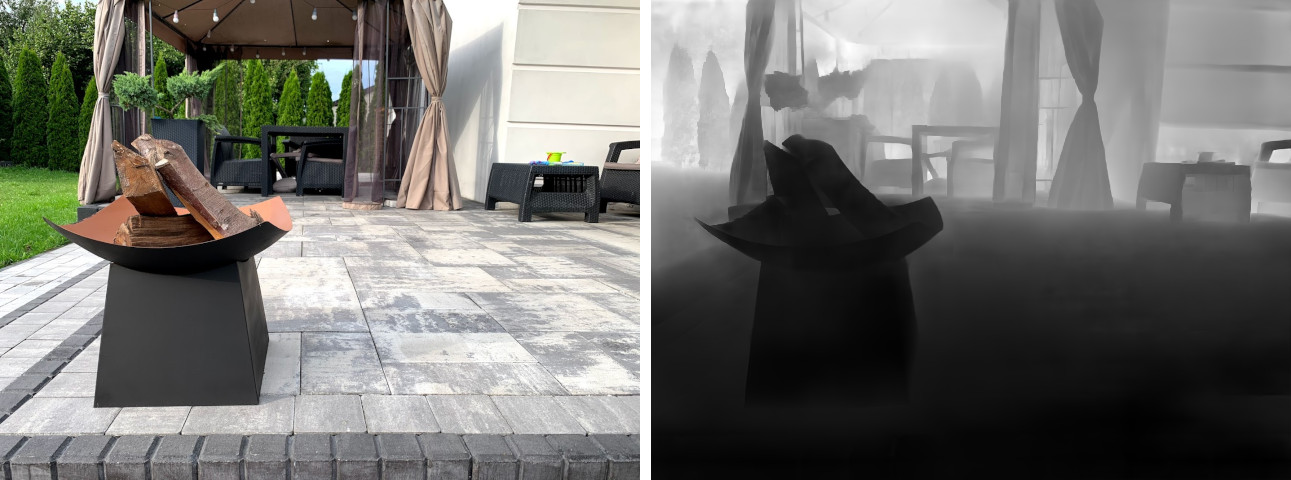
\includegraphics[width=0.9\textwidth]{1.jpg}
        \caption{Fotografia i odpowiadająca jej mapa głębi. Źródło: własne}
        \label{fig:depthmap}
 \end{figure}

W celu sprawnego funkcjonowania sieci neuronowej należy pierwotnie wykonać jej uczenie. Uczenie to polega na wyznaczeniu wag i parametrów danej sieci poprzez wykonanie algorytmu na zbiorze danych składającym się ze zbioru uczącego i zbioru testowego. Wyniki działania algorytmu na elementach zbioru uczącego porównywane są z odpowiadającymi tym elementom danymi o głębi zmierzonymi odpowiednią aparaturą podczas przygotowywania zbioru danych. Na podstawie tych porównań w kolejnych iteracjach wykonania algorytmu wagi oraz parametry są dopasowywane w taki sposób, aby wyniki następnych wykonań były jak najdokładniejsze. Najczęściej stosowanymi zbiorami danych w domenie głębi obrazu są NYU-Depth V2 \cite{couprie2013} zawierający 407024 obrazów uczących przedstawiających sceny wewnątrz budynków zarejestrowanych przy pomocy urządzenia Microsoft Kinect oraz KITTI (Karlsruhe Institute of Technology and Toyota Technological Institute) \cite{geiger2012} zawierający 93 tysiące obrazów uczących przedstawiających sceny zewnętrzne zarejestrowanych przy pomocy urządzenia z systemem LIDAR.

Pierwszą implementację omawianego algorytmu w 2014 r. zaproponowali pracownicy naukowi Instytutu Nauk Matematycznych Uniwersytetu w Nowym Jorku - David Eigen, Christian Puhrsch oraz Rob Fergus \cite{eigen2014}. Zaprojektowana wówczas przez wymienionych autorów architektura rozwiązania oparta została na dwóch współpracujących konwolucyjnych sieciach neuronowych \cite{oshea2015}. W dniu dzisiejszym osiągające najlepsze wyniki algorytmy również stosują w swojej architekturze sieci konwolucyjne, chociaż w kwestii częstości implementacji nie ustępują im na tym polu także transformatory \cite{vaswani2017}, które stanowią obecnie około połowę najczęściej używanych rozwiązań.

\section{Cel i układ pracy}
Aktualnie w otwartych źródłach istnieje wiele gotowych realizacji algorytmów percepcji głębi zdywersyfikowanych pod kątem architektury, funkcjonalności, osiąganych wyników i przeznaczenia. Wobec powyższego, celem badawczym niniejszej pracy inżynierskiej jest ich kompleksowa analiza porównawcza w ujednoliconym środowisku testowym.

Do realizacji nadrzędnego celu pracy przyjęto następujące zadania badawcze:
\begin{itemize}
    \item przegląd i ogólna charakterystyka dostępnych rozwiązań,
    \item wybór wiodących rozwiązań,
    \item weryfikacja metod na zbiorach, na których były uczone oraz na innych zbiorach,
    \item weryfikacja na własnych scenach,
    \item porównanie rozwiązań i rekomendacja przypadków użycia.
\end{itemize}

